\documentclass[10pt,letterpaper,addpoints]{exam}
\usepackage[utf8]{inputenc}
\usepackage[spanish,es-noshorthands]{babel}
\usepackage{hyperref}
\usepackage{amsmath}
\usepackage{amsfonts}
\usepackage{amssymb}
\usepackage{graphicx}
\usepackage{tikz}
\usepackage{multicol}
\usepackage[width=7in,height=9.5in]{geometry}
%\printanswers
\begin{document}
\title{\begin{minipage}{.2\textwidth}
        
\includegraphics[height=1.75cm]{Images/logo-colegio.png}
       \end{minipage}
\begin{minipage}{.55\textwidth}
 \begin{center}
Prueba bimestral ii\\Matemáticas $6^{\circ}$
\end{center}
\end{minipage}
\begin{minipage}{.2\textwidth}

\includegraphics[height=1.75cm]{Images/logo-sed.png} 
\end{minipage}
}
\author{Germ\'{a}n Avendaño Ram\'{i}rez\\Lic. Matemáticas U.D., M.Sc. U.N.}
\date{}
\maketitle
\begin{center}
\fbox{\fbox{\parbox{5.5in}{\centering
Conteste en el cuadro de respuestas rellenando los óvalos completamente. Puede usar una hoja de operaciones aparte.}}}
\end{center}
\vspace{0.1in}
\makebox[\textwidth]{Nombres: \hrulefill, curso:\underline{\hspace{48pt}}, fecha:\underline{\hspace{3cm}}}

\begin{multicols}{2}
\uplevel{Los relojes muestran las horas de iniciación y terminación del recreo en un colegio.}
\begin{center}
 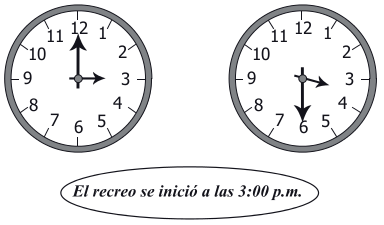
\includegraphics[scale=.55]{Images/relojes.png}
 \end{center} 
\begin{questions}
\question El recreo finalizó a las 3:30 p.m. ¿Cuánto avanzó el minutero desde que se inició el recreo?
\begin{choices}
\choice Un cuarto de vuelta.
\CorrectChoice Media vuelta.
\choice Tres cuartos de vuelta.
\choice Una 30 vuelta.
\end{choices}
\question Pepe tiene el doble de canicas que Luis y entre los dos reúnen 30 canicas. ¿Cuántas canicas tiene Pepe y cuántas canicas tiene Luis?
\begin{choices}
\choice Pepe tiene 6 canicas y Luis tiene 5 canicas.
\choice Pepe tiene 15 canicas y Luis tiene 15 canicas.
\CorrectChoice Pepe tiene 20 canicas y Luis tiene 10 canicas.
\choice Pepe tiene 60 canicas y Luis tiene 30 canicas.
\end{choices}
\question En la clase de matemáticas, la profesora Inés presenta las siguientes cuatro fichas marcadas con algunos dígitos para que los niños formen números:
\begin{center}
\begin{tikzpicture}
\draw (0,0) rectangle node{2} (.5,.5);
\draw (.6,.4) rectangle node{3} (1.1,.9);
\draw (.7,-.3) rectangle node{7} (1.2,.2);
\draw (1.4,-.1) rectangle node{0} (1.9,.4);
\end{tikzpicture}
\end{center}
¿Cuál es el mayor de los números de tres dígitos que los niños pueden formar con las fichas?
\begin{multicols}{2}
\begin{choices}
\choice 327
\choice 372
\CorrectChoice 732
\choice 735
\end{choices}
\end{multicols}
\uplevel{RESPONDE LA PREGUNTA ~\ref{q-01} DE ACUERDO CON EL SIGUIENTE TEXTO\\

Los estudiantes de grado quinto votaron para escoger la actividad con la que participarán en la celebración del Día del Colegio.}
\begin{center}
\begin{tabular}{|c|c|c|}
\hline 
 & \multicolumn{2}{c|}{Curso} \\ 
\hline 
\textbf{Actividad} & \textbf{Quinto A} & \textbf{Quinto B} \\ 
\hline 
Danza & 10 & 6 \\ 
\hline 
Teatro & 7 & 10 \\ 
\hline 
Canto & 9 & 9 \\ 
\hline 
Poes\'{i}a & 4 & 5 \\ 
\hline 
\end{tabular} 
\end{center}
Los estudiantes de grado quinto votaron para escoger la actividad con la que participarán en la celebración del Día del Colegio.
\question \label{q-01}
¿Cuál o cuáles de las siguientes afirmaciones, acerca de la votación de los estudiantes de grado quinto, es o son verdadera(s)?
\begin{itemize}
\item[I.] La actividad favorita de Quinta A es el canto.
\item[II.] La actividad favorita de Quinta B es el teatro.
\item[III.] El número de niños que prefieren la poesía en Quinto A y en Quinto B es el mismo.
\end{itemize}
\begin{multicols}{2}
\begin{choices}
\choice I solamente
\CorrectChoice II solamente
\choice I y III solamente
\choice II y III solamente
\end{choices}
\end{multicols}
\uplevel{La siguiente gráfica muestra la ubicación de diferentes atracciones de un parque de diversiones.
\begin{center}
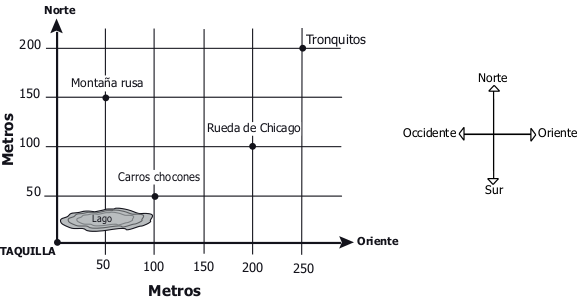
\includegraphics[scale=.45]{Images/grafica.png} 
\end{center}
}
\question Manuela está en la taquilla. Para llegar a los carros chocones ella debe caminar
\begin{choices}
\choice 50 metros al oriente y 150 metros al norte
\CorrectChoice 100 metros al oriente y 50 metros al norte
\choice 200 metros al oriente y 100 metros al norte
\choice 250 metros al oriente y 200 metros al norte
\end{choices}
\question La siguiente figura representa un caja. En la figura se señalan las dimensiones de la caja
\begin{center}
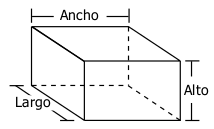
\includegraphics[scale=.75]{Images/caja.png} 
\end{center}
¿Cuál de los siguientes procedimientos permite hallar el volumen de la caja?
\begin{choices}
\choice Sumar el largo, el ancho y el alto de la caja.
\choice Multiplicar por 3 el alto de la caja.
\CorrectChoice Multiplicar el largo por el ancho y por el alto.
\choice Sumar el largo con el ancho, y multiplicar por el alto.
\end{choices}
\question Daniela quiere armar un cuadrado con algunas piezas. Hasta ahora, ha armado la siguiente figura:
\begin{center}
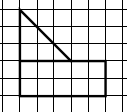
\includegraphics[scale=.75]{Images/figura06_03.png} 
\end{center}
¿Cuál de las siguientes piezas debe utilizar Daniela para terminar de armar el cuadrado?
\begin{center}
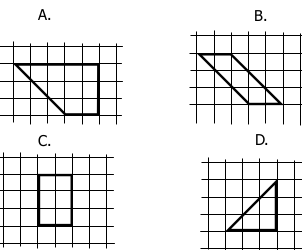
\includegraphics[scale=.75]{Images/figuras_06_03.png} 
\end{center}
\uplevel{RESPONDE LAS PREGUNTAS \ref{q-02} Y \ref{1-03} DE ACUERDO CON LA SIGUIENTE INFORMACIÓN\\

En una dulcería se elaboraron distintos empaques para vender dulces. Observa los dibujos.
\begin{center}
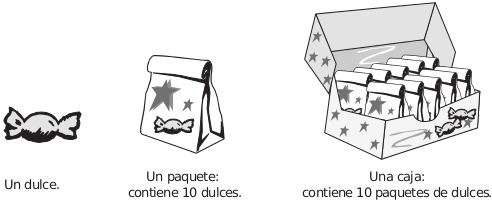
\includegraphics[scale=.5]{Images/dulces.png} 
\end{center}
}
\question \label{q-02}
Doña María quiere comprar quinientos ochenta y cuatro dulces. ¿Cuántas cajas, paquetes y dulces sueltos puede comprar doña María?
\begin{choices}
\choice 4 cajas, 8 paquetes y 5 dulces sueltos.
\choice 8 cajas, 5 paquetes y 4 dulces sueltos.
\CorrectChoice 5 cajas, 8 paquetes y 4 dulces sueltos.
\choice 5 cajas, 4 paquetes y 8 dulces sueltos.
\end{choices}
\question \label{q-03}
Don Pedro compró 2 paquetes de dulces, 4 cajas de dulces y 5 dulces sueltos. ¿Cuántos dulces compró en total?
\begin{multicols}{2}
\begin{choices}
\choice 10
\choice 245
\CorrectChoice 425
\choice 542
\end{choices}
\end{multicols}
\question En la siguiente tabla se muestra la cantidad de dinero que recibe el conductor de un bus, según el número de pasajeros que suben al bus.
\begin{center}
\begin{tabular}{|c|c|}
\hline 
\textbf{Número de pasajeros} & \textbf{Cantidad de dinero} \\ 
\hline 
3 & \$3\,600 \\ 
\hline 
4 & \$4\,800 \\ 
\hline 
5 & \$6\,000 \\ 
\hline 
• & • \\ 
\hline 
\end{tabular} 
\end{center}
¿Cuánto dinero recibe el conductor por un pasaje?
\begin{multicols}{2}
\begin{choices}
\choice \$600
\CorrectChoice \$1\,200
\choice \$1\,800
\choice \$3\,600
\end{choices}
\end{multicols}
\question El siguiente dibujo muestra la organización de los pupitres dobles en un salón:
\begin{center}
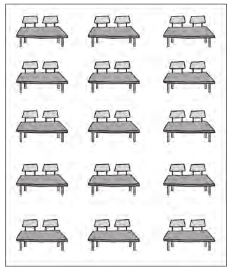
\includegraphics[scale=.75]{Images/sillas.png} 
\end{center}
¿Con cuál de las siguientes operaciones se puede hallar el número de sillas que hay en ese   salón?
\begin{multicols}{2}
\begin{choices}
\choice $5\times 3+2$
\CorrectChoice $5\times 3 \times 2$
\choice $(5+3)\times 2$
\choice $5\times (3+2)$
\end{choices}
\end{multicols}
\question La expresión $3\times (2+1)=6+3$ es
\begin{choices}
\CorrectChoice verdadera, porque $3\times (2+1)=9$ y $6+3=9$.
\choice falsa, porque $3\times (2+1)=6+1$
\choice verdadera, porque $2+1=3$ y $3+3=6$
\choice falsa, porque $2+1=3$ y $6+3=9$.
\end{choices}
\uplevel{Un número es primo si y sólo sí es divisible por sí mismo y por 1}
\question ¿Cuál de los siguientes números es primo?

\begin{oneparchoices}
\choice 18
\choice 21
\CorrectChoice 23
\choice 27
\end{oneparchoices}
\question En la siguiente figura se representan las áreas que ocupan diferentes cultivos en un terreno:
\begin{center}
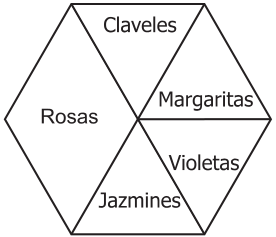
\includegraphics[scale=.5]{Images/claveles.png} 
\end{center}
La zona de los claveles ocupa un área de 10\,000 m$^{2}$. El área total del terreno es
\begin{multicols}{2}
\begin{choices}
\choice 10\,000 m$^{2}$
\choice 30\,000 m$^{2}$
\choice 50\,000 m$^{2}$
\CorrectChoice 60\,000 m$^{2}$
\end{choices}
\end{multicols}
\end{questions}
%cuadro de puntajes
%\begin{center}
%\gradetable[h][pages]
%\end{center}
\end{multicols}
\end{document}